\chapter{The Standard Model of Particle Physics}
\label{chap:sm}

\section{Introduction}

The Standard Model (SM) is a mathematical framework for the quantum mechanical description of matter and physical forces. It provides a description of the weak, strong, and electromagnetic interactions as mediated via ``messenger'' particles (gravity has so far eluded a quantum mechanical description). The particles constituting matter can be classified as \textit{quarks} or \textit{leptons} - quarks participate in the weak and strong force, leptons participate in the weak force; any charged particle experiences the electromagnetic force. \textit{Gauge bosons} are the particles responsible for the force interactions. The Higgs field is important for the generation of particle mass. This particle content has been seen in Figure~\ref{fig:sm}, we now turn to the field theory approach for these objects.

Matter particles are massive spin-1/2 fermions which are represented by solutions to the free-particle Dirac equation generated by the following Lagrangian, with equation of motion:

\begin{equation}
\begin{array}{l}
\mathcal{L} = i\bar{\psi}\gamma^{\mu}\partial_{\mu}\psi - m\bar{\psi}\psi\\
i\gamma^{\mu}\partial_{\mu}\psi - m\psi = 0
\end{array}
\end{equation}
respectively.

Particle interactions are generated by requiring the free-particle Lagrangian to be invariant under the action of different symmetry groups. Demanding local (gauge) invariance requires one to introduce spin-1 vector fields to the Lagrangian which couple with the fermions. The vector fields are to be identified with the generators of the symmetry group and act as the mediator of the force via particle exchange. U(1) generates electromagnetism via interactions with photons. A combination of U(1) and SU(2) generates the electroweak theory, simultaneously describing the electromagnetic and weak nuclear force via interactions with W$^{\pm}$ bosons, Z bosons and photons. SU(3) generates quantum chromodynamics, the theory of the strong nuclear force via interactions with gluons. These massive spin-1 gauge bosons are represented by solutions to the free particle Proca equations generated by the following Lagrangian, with equation motion:

\begin{equation}
\begin{array}{l}
\mathcal{L} = -\frac{1}{16\pi} \mathrm{B}^{\mu\nu}B_{\mu\nu} + \frac{1}{8\pi}m^{2}\mathrm{B}_{\nu}\mathrm{B}^{\nu}\\
\partial^{\mu} \partial_{\mu} \psi - m^{2} \psi = 0
\end{array}
\end{equation}
where $\mathrm{B}_{\mu\nu} \equiv \partial_{\mu}\mathrm{B}_{\nu} + \partial_{\nu}\mathrm{B}_{\mu}$ is known as the \textit{energy-momentum tensor} representing the kinetic energy of the field.

The mathematical fields which are contained with the SM are seen in Table~\ref{tab:sm}. This table will serve as a reference for the remainder of the chapter.

\begin{table}
\caption{Summary of field content within the SM.}
\centering
\begin{tabular}{c|ll}
\hline\hline
Gauge Sector & Matter Fields & Gauge Fields \\
%\hdashline
\hline
\textbf{SU(3)} & u, d, c, s, t, b & G$_{\mu}^{1...8} \rightarrow g_{\mu}^{1...8} $ \\
\hline
 & Q$_{L}$ = $\begin{pmatrix} u \\ d \end{pmatrix}_{L}, \begin{pmatrix} s \\ c \end{pmatrix}_{L}, \begin{pmatrix} t \\ b_{L} \end{pmatrix}_{L} $ & W$^{012}_{\mu}$, B$^{0}_{\mu}$ \\
\textbf{SU(2) $\times$ U(1)} & q = u, d, c, s, t, b & W$_{\mu}^{0}$, B$_{\mu}^{0}$ $\rightarrow$ Z$^{0}_{\mu}$, A$^{0}_{\mu}$\\
  & L$_{L}$ = $\begin{pmatrix} \nu_{e} \\ e^{-} \end{pmatrix}_{L} , \begin{pmatrix} \nu_{\mu} \\ \mu^{-} \end{pmatrix}_{L} , \begin{pmatrix} \nu_{\tau} \\ \tau^{-}\end{pmatrix}_{L} $ & W$_{\mu}^{1}$, W$^{2}_{\mu}$ $\rightarrow$ W$_{\mu}^{+}$, W$_{\mu}^{-}$\\
  & $\ell = (e, \mu, \tau)$ & \\
  \hline
\textbf{Higgs Sector} & $H = \begin{pmatrix} H^{+} \\ H^{0} \end{pmatrix} \rightarrow h^{0}$ & \\
  \hline\hline
\end{tabular}
\label{tab:sm}
\end{table}

\section{Quantum Electrodynamics}

Quantum electrodynamics describes the interactions of particles with electric charge. Beginning with a free-particle Dirac fermion we see the Lagrangian is invariant under the following U(1) transformation:

\begin{equation}
\psi(x)  \xrightarrow[]{\text{U(1)}} e^{i q \alpha}\,\psi(x)
\label{eq:u1}
\end{equation}
where $q$ is the electric charge, and $\alpha$ is an arbitrary constant.

In light of this symmetry, Noether's theorem implies the existence of a conserved (electromagnetic) current $j^{\mu} = -e\bar{\psi}\gamma^{\mu}\psi$ ($\partial_{\mu}j^{\mu}=0$). If we then allow the U(1) transformation to be space-time dependent, that is $\alpha = \alpha(x)$, we must introduce a new spin-1 vector field A$^{\mu}$ in order for the derivative to transform such that the Lagrangian remain invariant. This new field in introduced by making a redefinition of the partial derivate, called the \textit{covariant derivative}, and the following transformation property for the new field:

\begin{equation}
\begin{array}{l}
\partial{\mu} \rightarrow\ \partial_{\mu} - ie\mathrm{A}_{\mu}
\\A_{\mu} \xrightarrow[]{\text{U(1)}} \mathrm{A}_{\mu} + \frac{1}{e} \partial_{\mu} \alpha
 \end{array}
\end{equation}

We then make the substitution into the Lagrangian:
\begin{equation}
\mathcal{L}_{\mathrm{QED}} =
i\bar{\psi}\gamma^{\mu}\partial_{\mu}\psi
- e\bar{\psi}\gamma^{\mu}\psi \mathrm{A}_{\mu}
- m\bar{\psi}\psi
- \frac{1}{4}\mathrm{F}_{\mu\nu} \mathrm{F}^{\mu\nu}
\end{equation}

where $\mathrm{F}_{\mu\nu}\equiv\partial_{\mu}\mathrm{A}_{\nu} - \partial_{\nu}\mathrm{A}_{\mu}$ is the field strength tensor.

We see that in order for the Lagrangian to remain invariant under this U(1) transformation, we were forced to introduce an additional term which links the conserved electromagnetic current with the spin-1 field: $e\bar{\psi}\gamma^{\mu}\psi \mathrm{A}_{\mu} = j^{\mu}A_{\mu}$. This new field is to be identified with the photon,  it acts as a mediator of the force between two particles with electric charge. A photon mass term of the form $\frac{1}{2}m^{2}\mathrm{A}^{\mu}\mathrm{A}_{\mu}$ is forbidden as it is not invariant under the transformation rule, the photon remains massless.

\section{Quantum Chromodynamics} 

Quantum chromodynamics describes the interactions of quarks due to the strong nuclear force. The theory is generated by demanding local invariance of the Lagrangian under an SU(3) symmetry operating on \textit{color triplets}. Eight new gauge fields must be introduced to give the proper transformation rule of the covariant derivative. These new gauge fields become the gluons and act as the mediator of the strong force, mixing the color states within a quark.

Consider the following SU(3) transformation:
\begin{equation}
q_{c} \xrightarrow[]{\text{SU(3)}} e^{ \frac{1}{2} i g_{s} \bm{\xi}(x) \cdot \bm{\lambda}} \, q_{c}
\end{equation}
where $g_{s}$ is the strong coupling constant, $\bm{\xi}$ is an 8-dimensional vector of arbitrary functions of spacetime, $\bm{\lambda}$ are the 8 3x3 Gell-Mann matrices, and $\overline{q_{c}}=(\overline{q_{red}}, \overline{q_{green}}, \overline{g_{blue}})$ is a color-triplet such that $q(x) = q_{c} q_{D}(x)$ and $q_{D}(x)$ is a Dirac fermion (any of the 6 SM quarks).

SU(3) gauge invariance requires us to modify the definition of the partial derivative to include 8 spin-1 vector fields $\bm{\mathrm{G}}_{\mu}$:
\begin{equation}
\begin{array}{l}
\partial{\mu} \rightarrow \partial_{\mu} - i g_{s} \bm{\lambda} \cdot \bm{G}_{\mu}\\
G^{k}_{\mu} \xrightarrow[]{\text{SU(3)}} G^{k}_{\mu} - \frac{1}{g_{s}}\partial_{\mu}\xi_{k} - f_{ijk}\xi_{i}G^{j}_{\mu}
\end{array}
\end{equation}
where $f_{ijk}$ are known as the \textit{structure constants} of SU(3) and arise from its non-abelian nature, they satisfy $[\lambda_{i},\lambda_{j}] = 2if_{ijk}\lambda_{k}$.

The complete Lagrangian becomes:
\begin{equation}
\mathcal{L}_{\mathrm{QCD}} =
i \bar{q} \gamma^{\mu} \partial_{\mu} q
-  \frac{1}{2} (g_{s} \bar{q} \gamma^{\mu} \bm{\lambda} q) \cdot \textbf{G}_{\mu}
- m \bar{q} q
- \frac{1}{4} \textbf{G}^{\mu\nu} \cdot \textbf{G}_{\mu\nu}
\end{equation}

where $\mathrm{G}^{\mu\nu}_{i} \equiv \partial^{\mu} \mathrm{G}^{\nu}_{i} - \partial^{\nu} \mathrm{G}^{\mu}_{i} - g_{s} f_{ijk} \mathrm{G}^{\mu}_{j} \mathrm{G}^{\nu}_{k}$ is the field strength tensor for the gluon field $i$. We see the non-abelian nature of SU(3) manifests itself as self-couplings within the gluon field, giving rise to interaction vertices with 3 or 4 gluons. 8 conserved color currents, analogous to the electromagnetic current, are seen as interaction terms between two quarks and a gluon $(\frac{1}{2} g_{s} \bar{q} \gamma^{\mu} \bm{\lambda} q) \cdot \bm{\mathrm{G}}_{\mu} = \bm{j}^{\mu} \cdot \bm{\mathrm{G}}_{\mu}$.

To conserve color charge at the QCD vertices, gluons themselves must carry both color and anti-color. The color charge allows for self interactions of the gluons (contrast with the  to the elec. The 8 physical gluons are members of a color/anticolor octet. 6 of them are expressed as ladder operators within SU(3) and the other two are diagonal matrices.

A gluon mass term of the form $\frac{1}{2}m^{2}\bm{\mathrm{G}}^{\mu} \cdot \bm{\mathrm{G}}_{\mu}$ is forbidden as it is not invariant under the transformation rule, the gluons remain massless.

\subsection{Confinement, Hadrons, \& the Quark Model}

Experimentally we have never detected a free quark. The physical manifestation of quark production results in a final state consisting of many lower energy particles produced collinear with the original quark. This ``spray'' of particles is known as a \textit{jet}. This behavior can be explained if one accepts the hypothesis of \textit{color confinement} stating that all objects with color charge are confined to colorless singlets. The origins of color confinement may be traced to the self interactions of the gluon fields resulting in the strong force between two quarks to \textbf{increase} as they separate. It eventually becomes energetically favorable to create quark-antiquark pairs from the vacuum which can subsequently combine with other quarks to form the colorless objects (constituting the jets).

\textit{Hadrons} are bound states of quarks which interact through the strong force. Color confinement limits the possible combinations of quarks and antiquarks which can exist together in a bound state (antiquarks carry anticolor). Among states consisting of two quarks+antiquarks, the only possible color singlet wave function is a $q\bar{q}$ pair: $\psi = \frac{1}{\sqrt{3}} (r\bar{r} + g\bar{g} + b\bar{b})$ - these states are called \textit{mesons}. For systems of three quarks+antiquarks, the only color singlet consists of three quarks $qqq$: $\psi = \frac{1}{\sqrt{6}} (rgb - rbg + gbr - grb +brg-bgr)$ - these states are called \textit{baryons}.

The strength of the strong force between two quarks is independent of their flavor and therefore QCD possesses a symmetry under rotations in flavor-space. This would be an exact symmetry if it were not for the physical quark masses (Figure \ref{fig:sm}). To a crude approximation the $u$, $d$, and $s$ quarks have the same mass: 2.2, 4.7, and 96 MeV, (compare to the $c$ with a mass of 1.28 GeV). The $uds$ quarks can therefore be thought of as different states within a triplet. This is known as the \textit{SU(3) flavor symmetry}. Within the symmetry, the $q\bar{q }$ meson states can be combined to form two nonets with angular momentum $l=0$, and spins of $s=0$ or $s=1$. The $s=0$ states are the lowest energy and provide a quark description of the kaons and pions. The $qqq$ baryons can form flavor states consisting of a $j=1/2$ octet and $j=3/2$ decuplet. The $j=1/2$ states are the lowest energy and describe the proton and neutron. These multiplet structures can be seen in Figure~\ref{fig:su3flavor}. 

\begin{figure}[hbp!]
\centering
\begin{subfigure}[c]{0.425\textwidth}
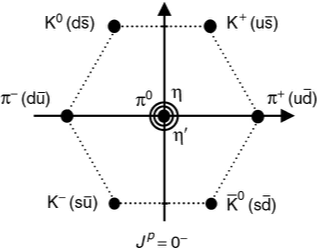
\includegraphics[width=0.95\textwidth]{figs/mesons.png}
\caption{Two quark bound states ($l=s=0$).}
%\label{fig:t5hh}
\end{subfigure}
\begin{subfigure}[c]{0.425\textwidth}
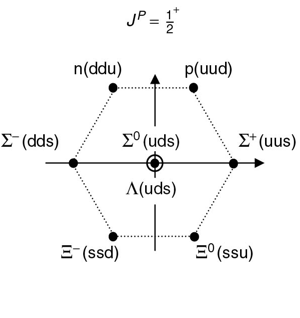
\includegraphics[width=0.95\textwidth]{figs/baryons.png}
\caption{Three quark bound states ($l=0, s=1/2$).}
\end{subfigure}
\caption{SU(3) flavor symmetry multiplets predicted by the quark model.}
\label{fig:su3flavor}
\end{figure}

\section{Electroweak Theory} 

\subsection{Introduction}

The electroweak theory provides a unified and self-consistent description of both the electromagnetic and weak forces. The complete theory is generated by demanding local invariance of the Lagrangian under a combined SU(2)$\times$U(1) symmetry. The SU(2) invariance requires the addition of three new vector bosons, two of which are used to construct the physical W$^{\pm}$ bosons responsible for the weak \textit{charged current} interactions. An additional gauge boson is required for the U(1) symmetry. A mixing between the remaining (neutral) SU(2) gauge field and the U(1) gauge field yield the Z boson and photon, responsible for weak \textit{neutral current} and electromagnetic interactions, respectively. 

Consider the following U(1) transformation on a fermion $\psi$, and SU(2) transformation on an \textit{isospin doublet} $\Psi$:

\begin{equation}
\begin{array}{l}
\psi(x) \xrightarrow[]{\text{U(1)}} e^{i g' \frac{Y}{2} \alpha(x)} \, \psi(x) \\
\Psi(x) \xrightarrow[]{\text{SU(2)}} e^{i g_{W} \bm{\xi}(x) \cdot \frac{1}{2} \bm{\sigma} } \, \Psi(x) 
\end{array}
\end{equation}
where $g'$ is the hypercharge coupling constant, Y is the hypercharge operator, $g_{W}$ is the weak coupling constant, $\alpha$ and $\bm{\xi}$ are arbitrary functions of spacetime, and $\bm{\sigma}$ represents the 3 2x2 Pauli spin matrices.

As usual, SU(2) and U(1) gauge-invariance requires us to modify the definition of the partial derivate to include three spin-1 vector fields $\bm{\mathrm{W}}^{\mu}$ and a single spin-1 vector field B$^{\mu}$:

\begin{equation}
\begin{array}{l}
\partial{\mu} \rightarrow\ \partial_{\mu} - i g' \frac{Y}{2}\mathrm{B}_{\mu} -  i g_{W} \frac{1}{2}\bm{\sigma} \cdot \bm{\mathrm{W}}_{\mu}\\
\mathrm{B}_{\mu} \xrightarrow[]{\text{U(1)}} \mathrm{B}_{\mu} - i g' \partial_{\mu} \alpha \\
\mathrm{W}^{k}_{\mu} \xrightarrow[]{\text{SU(2)}} \mathrm{W}^{k}_{\mu} - g_{W} \partial_{\mu} \xi^{k} -  g_{W} \epsilon_{ijk} \xi^{i} \mathrm{W}^{j}_{\mu}
 \end{array}
\end{equation}
where $\epsilon_{ijk}$ is the totally antisymmetric Levi-Civita tensor (the structure constants of SU(2)).

The charged current interaction connects two elements within an isospin doublet $\Psi$; by convention, the upper element has electric charge +1 relative to the lower element. There are doublets which connect the leptons with a corresponding neutrino (massless spin-1/2 particles), and there are doublets which connect an 'up-type' quark (top entry of the doublet) to a 'down-type' quark (bottom entry):

\begin{equation*}
\begin{pmatrix} \nu_{e} \\ e^{-} \end{pmatrix},
\begin{pmatrix} \nu_{\mu} \\ \mu^{-} \end{pmatrix},
\begin{pmatrix} \nu_{\tau} \\ \tau^{-} \end{pmatrix},
\begin{pmatrix} u \\ d' \end{pmatrix},
\begin{pmatrix} c \\ s' \end{pmatrix},
\begin{pmatrix} t \\ b' \end{pmatrix}
\end{equation*}

The W$^{1}$ and W$^{2}$ gauge fields correspond to the first two Pauli matrices; appropriate linear combinations of these two fields therefore define raising and lowering operators which transform elements within a doublet. The physical W$^{\pm}$ bosons are the following linear combinations of the two gauge fields:
\begin{equation}
\mathrm{W}_{\mu}^{\pm} = \frac{1}{\sqrt{2}} ( \mathrm{W}^{1}_{\mu} \mp i\mathrm{W}_{\mu}^{2})
\end{equation}

As Nature has it, the weak force is a \textit{chiral} theory which does not treat the left and right-chiral components of a Dirac fermion on equal footings.  The projection operator $P_{R/L} = \frac{1}{2} ( 1 \pm \gamma^{5})$ is used to define these left and right chiral states, all Dirac fermions can be decomposed as $\psi = \psi_{L} + \psi_{R}$ using these operators. In the Standard Model, only left-handed particle and right-handed antiparticle states enter into the isospin doublets participating in the electrically-charged weak interaction. This is summarized in Table~\ref{tab:sm}.

Because of the SU(2) symmetry and doublet nature, we must introduce \textbf{two} fermions to the theory, where the left and right chiral components may transform differently under gauge interactions. Consider fields  $\chi$ and  $\tau$; the left handed components are members of an isospin doublet $\overline{\psi_{L}}=(\overline{\chi_{L}},\,\overline{\tau_{L}})$, all components participate in the U(1) transformation. The complete Lagrangian becomes:

\begin{equation}
\begin{array}{l}
\mathcal{L}_{\mathrm{EWK}} = 
i \bar{\chi} \gamma^{\mu} \partial_{\mu} \chi - m \bar{\chi} \chi
+ i \bar{\tau}   \gamma^{\mu}    \partial_{\mu} \tau  - m \bar{\tau} \tau
- \frac{1}{4}\mathrm{B}_{\mu\nu}\mathrm{B}^{\mu\nu}
-\frac{1}{4}\bm{\mathrm{W}}_{\mu\nu} \cdot \bm{\mathrm{W}}^{\mu\nu} \\
\hspace{1.2cm}
-  g' \bar{\chi} \gamma^{\mu} \frac{Y}{2} \chi \mathrm{B}_{\mu} + g' \bar{\tau} \gamma^{\mu} \frac{Y}{2} \tau \mathrm{B}_{\mu}
- g_W  \overline{\psi_{L}} \gamma^{\mu} \bm{\sigma} \psi_{L} \cdot \bm{\mathrm{W}}_{\mu}
\end{array}
\end{equation}

Mass terms of the form $\frac{1}{2}m^{2}\mathrm{A}^{\mu}\mathrm{A}_{\mu}$ are forbidden as they are not invariant under the transformation rule, the B and $\bm{\mathrm{W}}$ bosons remain massless.

\subsection{The Higgs Mechanism}

The gauge bosons responsible for the electroweak force have observationally been determined to have mass, which is a problem as the gauge symmetry requires them to be massless. Surely there must be some mechanism which can be introduced to achieve this meanwhile (at least initially) preserving the SU(2)$\times$U(1) symmetry. The \textit{Higgs field} is introduced to generate mass terms for the electroweak gauge bosons. The discovery of the Higgs boson was the final particle contained within the SM to be observed, its discovery in 2012 was monumental.\cite{higgsdisc}

This Higgs mechanism proceeds by introducing a massive spin-0 complex scalar field with the following Lagrangian:
\begin{equation}
\label{higgslag}
\mathcal{L} = \frac{1}{2} (\partial_{\mu}\phi^{\dagger})(\partial^{\mu}\phi) - \frac{1}{2}\mu^{2} \phi^{\dagger}\phi + \lambda(\phi^{\dagger}\phi)^{2}
\end{equation}
where $\mu$ and $\lambda$ are the strengths of the self-coupling terms.

Within the SM, the field is implemented as an isospin doublet which consists of electrically neutral and charged components:
\begin{equation}
\phi = \begin{pmatrix} \phi^{+} \\ \phi^{0} \end{pmatrix} = \begin{pmatrix} \phi_{1} + i\phi_{2} \\  \phi_{3} + i\phi_{4} \end{pmatrix},
\end{equation}

Solving for the minimum of the potential, it is found that the ground state of $\phi$ is non-zero and satisfies $\phi^{\dagger}\phi = \phi_{1}^{2} + \phi_{2}^{2} + \phi_{3}^{2}  + \phi_{4}^{2} = \frac{1}{2}v^{2} = - \mu^{2}/{2\lambda}$. This is called \textit{spontaneous symmetry breaking} - the Higgs acquiring a \textit{vacuum expectation value}. Perturbation theory of interactions represent particles as fluctuations above the vacuum - we must express the fields in the same manner. Electric charge conservation requires that this vacuum expectation value lie entirely inside the neutral $\phi^{0}$. This ground state is then expressed as: 
\begin{equation}
\phi = \begin{pmatrix} 0 \\  v + h(x) \end{pmatrix},
\end{equation}
where $h(x)$ is to be identified as the Higgs boson.

If we substitute the ground-state expansion of $\phi$ to the Lagrangian of Equation \ref{higgslag} we obtain the following expression:
\begin{equation}
\mathcal{L} = \frac{1}{2}(\partial^{\mu}h)(\partial_{\mu}h) - \lambda v^{2} h^{2} - \lambda vh^{3} - \frac{1}{4}\lambda h^{4} + \lambda v^{4}
\end{equation}
where we see have generated a mass term $m_{\mathrm{h}} = \sqrt{2 \lambda} v$ for the Higgs boson, additionally there are now 3 and 4-point Higgs self-couplings.

\subsubsection{Masses of the W$^{\pm}$ and Z bosons}

The kinetic energy term $\frac{1}{2} (\partial_{\mu}\phi^{\dagger})(\partial^{\mu}\phi)$ for the Higgs field introduces a coupling with the $\bm{\mathrm{W}}^{\mu}$ and B$^{\mu}$ bosons when they are added to the covariant derivate:

\begin{equation}
\partial_{\mu}\phi = (\frac{1}{2}\partial_{\mu} + \frac{1}{2} i g_{W}\bm{\sigma}\cdot\bm{\mathrm{W}} + i g' \frac{Y}{2} \mathrm{B}^{\mu})\begin{pmatrix} 0 \\ v + h(x) \end{pmatrix}
\end{equation}

After performing the matrix calculations, and lots of algebra, there are terms quadratic in the gauge fields:
\begin{equation}
\frac{1}{8} v^{2} g_{\mathrm{W}}^{2} ( \mathrm{W}^{1}_{\mu} \mathrm{W}_{1}^{\mu} + \mathrm{W}^{2}_{\mu} \mathrm{W}_{2}^{\mu}) + \frac{1}{8} v^{2} ( g_{W} \mathrm{W}^{3}_{\mu} - g'\mathrm{B}_{\mu} ) ( g_{W} \mathrm{W}_{3}^{\mu} -g' \mathrm{B}^{\mu} )
\end{equation}

Where we see we have generated mass terms for the W$^{\mu}_{1}$ and W$^{\mu}_{2}$ fields:  $m_{\mathrm{W}} = \frac{1}{2} v g_{W}$. The last term in the expansion introduces mixed couplings between the electrically neutral and massless W$_{3}^{\mu}$ and B$^{\mu}$ fields. The mixing can be represented via a non-diagonal mass matrix. Physical particles propagate as independent eigenstates of the free particle Hamiltonian and therefore we must find the basis in which this matrix is diagonal. Upon diagonalization, we find the states corresponding to these eigenvalues:

\begin{equation}
\begin{array}{l}
A_{\mu} = \frac{1}{\sqrt{g_{W}^{2} + g'^{2}}} \, (g' \mathrm{W}^{3}_{\mu} + g_{W}\mathrm{B}_{\mu});\hspace{0.5cm} \mathrm{with\,\,mass}\,\,0\\
\mathrm{Z}_{\mu} = \frac{1}{\sqrt{g_{W}^{2} + g'^{2}}} \, (g_{W} \mathrm{W}^{3}_{\mu} - g'\mathrm{B}_{\mu}); \hspace{0.56cm} \mathrm{with\,\,mass}\,\, \frac{1}{2}v\sqrt{g_{W}^{2} + g'^{2}}
\end{array}
\end{equation}
where $\mathrm{A}_{\mu}$ corresponds to the photon of electromagnetism, and Z$_{\mu}$ the neutral gauge boson responsible for the weak neutral currents.

We have seen how the Higgs mechanism is able to generate mass terms for the gauge bosons in the electroweak theory.

\subsubsection{Masses of the Fermions}

It has not been mentioned that the fermion mass terms $-m\bar{\psi}\psi = -m( \overline{\psi_{R}} \psi_{L} + \overline{\psi_{L}}\psi_{R})$ are in fact forbidden within the SM - the chiral nature of SU(2) treats the two chiral states differently and therefore this term is not invariant under the transformation rules. Masses for the fermions are created by introducing \textit{Yukawa interactions} with the Higgs field. Consider the following terms which are invariant under the U(1)$\times$SU(2) transfomation:

\begin{equation}
\begin{array}{l}
\mathcal{L} = -y [ \overline{\psi_{L}} \, \phi \, \psi_{R} + \overline{\psi_{R}} \, \phi^{\dagger} \, \psi_{L}]\\
=  -y\left[\begin{pmatrix} \bar{\nu},\,\bar{\ell}\end{pmatrix}_{L} \begin{pmatrix} \phi^{+} \\ \phi^{0} \end{pmatrix} \ell_{R} + 
\overline{\ell_{R}} \begin{pmatrix} \phi^{+*},\,\phi^{0*} \end{pmatrix} \begin{pmatrix} \nu \\ \ell \end{pmatrix}_{L}\right]
\end{array}
\end{equation}
where $y$ is the \textit{Yukawa coupling}, $\overline{\psi_{L}}$ is an isospin doublet of left-chiral fermions, and $\psi_{R}$ is a right-chiral fermion.

After spontaneous symmetry breaking, this reduces to:

\begin{equation}
\begin{array}{l}
\mathcal{L} =
-\frac{1}{\sqrt{2}}yv (\overline{\ell_{L}}\ell_{R} + \overline{\ell_{R}}\ell_{L})
-\frac{1}{\sqrt{2}}yh (\overline{\ell_{L}}\ell_{R} + \overline{\ell_{R}}\ell_{L})\\
\hspace{4mm} = - \frac{1}{\sqrt{2}} yv \bar{\ell}\ell - \frac{1}{\sqrt{2}} y h \bar{\ell}\ell
\end{array}
\end{equation}
and we see we have obtained a mass term for the fermion $m_{\ell} = \frac{1}{\sqrt{2}} yv$ and an interaction term $\frac{1}{\sqrt{2}} y h \bar{\ell}\ell$ between the fermion in the lower member of the isospin double and a single Higgs boson.

To generate a mass term for the upper component of the isospin doublet we need to follow the same prescription but with the \textit{conjugate} Higgs field:

\begin{equation}
\phi_{c} = - i \sigma_{2} \phi^{*}
= \begin{pmatrix} -\phi^{0*} \\ \phi^{-} \end{pmatrix} = \frac{1}{\sqrt{2}} \begin{pmatrix} -\phi_{3} + i\phi_{4} \\  \phi_{1} - i \phi_{2} \end{pmatrix},
\end{equation}

where the same story plays out.

%%\begin{table}
%%\centering
%\caption{Quantum numbers of the electroweak SM.}
%\begin{tabular}{ r | cccc }
%\hline\hline
%particle & Q & I$^{3}_{W}$ & Y$_{L}$ & Y$_{R}$ \\
%\hline
%$\nu_{e}$, $\nu_{\mu}$, $\nu_{\tau}$ & 0 & +1/2 & -1 & 0 \\ 
% $e^{-}$, $\mu^{-}$, $\tau^{-}$ & -1 & -1/2 & -1 & -2 \\ 
%u, c, t & +2/3 & +1/2 & +1/3 & +4/3 \\ 
%d, s, b & -1/3 & -1/2 & +1/3 & -2/3 \\
%\hline
%Higgs & 0 & -1/2 & \multicolumn{2}{c}{+1}\\
%Z & 0 & 0 &  \multicolumn{2}{c}{0}\\
%A & 0 & 0 &  \multicolumn{2}{c}{0}\\
%W$^{\pm}$ & $\pm1$ & $\pm1$ &  \multicolumn{2}{c}{0}\\
%\hline\hline
%\end{tabular}
%\label{tab:ewkqn}
%\end{table}

\subsection{Quark Mixing - the CKM Matrix}

The charged weak current acts on isospin doublets connecting quarks of different flavors - the flavor eigenstates: u, d, s, c, b, t. The quarks propagate as mass eigenstates of the free-particle Hamiltonian. This introduces mixing between these two bases and is represented by the \textit{CKM matrix}. The probability of a transition between two states is proportional to a matrix element $|V|^{2}$ in the matrix. It is unitary 3x3 matrix with 4 degrees of freedom:

\begin{equation}
\label{eq:ckmv}
\begin{pmatrix} d' \\ s' \\ b' \end{pmatrix} =
\begin{pmatrix} V_{ud} \,\, V_{us}  \,\, V_{ub} \\ V_{cd} \,\, V_{cs} \,\, V_{cb}  \\ V_{td} \,\, V_{ts} \,\, V_{tb} \end{pmatrix}
\begin{pmatrix} d \\ s \\ b \end{pmatrix}
\end{equation}

The best estimate of these parameters are:

\begin{equation}
\label{eq:ckmval}
\begin{pmatrix} |V_{ud}| \,\, |V_{us}|  \,\, |V_{ub}| \\ |V_{cd}| \,\, |V_{cs}| \,\, |V_{cb}|  \\ |V_{td}| \,\, |V_{ts}| \,\, |V_{tb}| \end{pmatrix} \approx
\begin{pmatrix} 0.974 \,\, 0.225  \,\, 0.004 \\ 0.225 \,\, 0.973 \,\, 0.041  \\ 0.009 \,\, 0.040 \,\, 0.999 \end{pmatrix}
\end{equation}

\subsection{Brief Electroweak Summary}

We started with a theory of two fields each governed by the Dirac equation. We demanded that the theory be gauge-invariant under combined U(1)$\times$SU(2) symmetry operations. The gauge bosons are required to be massless as their transformation rules do not allow their kinetic energy term to be invariant. The Higgs field was introduced, the action of the covariant derivate on the Higgs field generates an interaction term between the gauge bosons and the Higgs field. The Higgs field obtained a vacuum expectation value, re-expressing the field about this ground state led us to mass terms for the gauge bosons. The physical W$^{\pm}$, Z, and A bosons become mixtures of these states. Fermion mass terms are not initially allowed as the chiral SU(2) symmetry treats the left and right-chiral components differently and therefore can not remain invariant. Fermion mass terms are generated by introducing Yukawa interactions between the Higgs field and fermions which generate appropriate mass terms after the Higgs field expansion. In addition, under the charged-current interaction, quark flavor and mass eigenstates are not the same, this introduces the CKM matrix parametrizing the mixing.

\section{Parameters of the Standard Model}

There are 18 parameters that must be specified as an input to the SM - these must all be determined experimentally:

\begin{itemize}
\item 9 quark and lepton masses: $m_{u}, m_{d}, m_{s}, m_{c}, m_{b}, m_{t}, m_{e}, m_{\mu}, m_{\tau}$; the values are listed in Figure~\ref{fig:sm}. (Alternatively these can be expressed as the 9 appropriate Yukawa couplings $y_{f}=\sqrt{2}m_{f} / v$: 1, 1, 1, 1, 1, 1, 1, 1, 1 respectively)
\item 4 parameters describing the mixing between quark mass and flavor eigenstates (CKM matrix, see Equations \ref{eq:ckmv} and \ref{eq:ckmval}): often parametrized as $\lambda, A, \rho, \eta$
\item 2 parameters for the Higgs field: mass and vacuum expectation value m$_{H}$ = 125 GeV, v = 246 GeV 
\item 3 coupling constants for the relative strengths of the gauge group:
\begin{equation*}
\begin{array}{ll}
\alpha \equiv e^{2} / 4 \pi, & \alpha(q^{2} \approx 0) = 1 / 137.0 \\
 & \alpha(q^{2} = (193\,\mathrm{GeV})^{2}) = 1 / (127.4\pm 2.1)\\
\alpha_{s} \equiv g_{s}^{2} / 4 \pi,  & \alpha_{s}(q^{2}=m_{Z}^{2} = (91\,\mathrm{GeV})^{2})= 0.1184 \pm 0.0007\\
G_{F} \equiv \sqrt{2} g^{2}_{W} / 8 m_{W}^{2}, & G_{F} (q^{2}\approx0) = 1.1663787\times10^{-5} \\

\end{array}
\end{equation*}
\end{itemize}

\section{Neutrino Mass}

Within the 'canonical' SM the neutrinos are assumed to be massless spin-1/2 fermions. In the last decade, experiments have shown that neutrinos go through \textit{flavor oscillations} wherein they change flavor as they propagate through space. This flavor oscillation is dependent on \textbf{massive} neutrinos and can be described by a mixing between these mass and flavor eigenstates. The mixing is described by a 3x3 unitary matrix known as the \textit{PMNS matrix} (analogous to the CKM matrix). One could consider giving the neutrinos a Yukawa coupling with the Higgs and give them a Dirac mass $-m\bar{\nu}\nu = -m(\overline{\nu_{R}}\nu_{L} + m\overline{\nu_{L}}\nu_{R})$, but the non-observation of right-handed neutrinos does not allow that approach. The correct implementation of the neutrino mass is still an open question in the field. The currently known estimates for their masses are seen in Figure~\ref{fig:sm}.

The neutrino mass sector possibly adds an additional 7 parameters to the SM:
\begin{itemize}
\item 3 neutrino masses: $m_{\nu_{1}}, m_{\nu_{2}}, m_{\nu_{3}}$
\item 4 parameters describing the mixing between the neutrino mass and flavor eigenstates (PMNS matrix): often parameterized as $\theta_{12}, \theta_{13}, \theta_{23}, \delta$.
\end{itemize}

The best fit values of the PMNS matrix are:
\begin{equation}
\begin{pmatrix} |U_{e1}| \,\, |U_{e2}|  \,\, |U_{e3}| \\ |U_{\mu1}| \,\, |U_{\mu2}| \,\, |U_{\mu3}|  \\ |U_{\tau1}| \,\, |U_{\tau2}| \,\, |U_{\tau3}| \end{pmatrix} \approx
\begin{pmatrix} 0.85 \,\, 0.50  \,\, 0.17 \\ 0.35 \,\, 0.60 \,\, 0.70  \\ 0.009 \,\, 0.35 \,\, 0.70 \end{pmatrix}
\end{equation}
